\chapter{Numerical Simulations of Limit Order Book using Poisson Processes}

\section{Introduction}
LOBs act as a mechanism for buyers and sellers to interact in financial markets. Today, most exchanges provide real-time data access. With the rise of algorithmic trading systems, the order book and its history have become one of the most utilized forms of financial data. 

\subsection*{The Necessity of LOB Modelling}

Modelling and simulating LOBs is necessary for several key reasons:

\begin{itemize}
    \item \textbf{Understanding Market Dynamics:} The time evolution of the order book captures the highly complex dynamics of supply and demand. 
    \item \textbf{Observing Price Formation:} The LOB allows researchers to observe the price formation of a security at the most granular level possible.
    \item \textbf{Gauging Liquidity:} The state of the order book serves as a strong indicator of market liquidity.
    \item \textbf{Testing and Calibration:} Simulating the order book lets practitioners replay history. This is essential for backtesting, calibrating, and fine-tuning automated algorithmic trading strategies.
\end{itemize}

The recent availability of faster and cheaper computing power has allowed these simulations to grow richer. Models are generally tested against empirical observations, known as stylized facts, to ensure their outputs reflect real-world market behavior. 

\subsection*{Methodologies in LOB Simulation}

The current state of the art features a wide variety of simulation techniques. These models broadly fall into two main categories: Point Process models and Deep Learning models. 

\subsubsection{Point Process Models}
Mathematically, an LOB is an aggregate of individual orders arriving at different times. Therefore, it is natural to model the order book as a queueing system using point processes. Because these models are mathematically descriptive, they are fully explainable.

\begin{itemize}
    \item \textbf{Poisson Processes:} Poisson models assume that order arrivals are independent of each other. Basic versions are ``zero-intelligence'' models because they use no prior expert heuristics or market information. Researchers have enhanced these models by making order arrival rates variable, depending on the current state of the queue. While mathematically convenient, the assumption that all orders are independent contradicts real market behavior. For example, Poisson models cannot explain the clustering effect of order events.
    \item \textbf{Hawkes Processes:} Hawkes processes solve the major challenges of Poisson models by relaxing the assumption of independent increments. Instead, they model order flow as an endogenously excited process. This means past events can trigger future events. A Hawkes process can have multiple dimensions to represent different order types, and these dimensions can excite one another. Because of this, Hawkes models successfully reproduce important structural details like volatility clustering and implicit market impact. While highly adaptable, their complex math makes calibration a key challenge.
\end{itemize}

\subsubsection{Deep Learning Based Models}
The LOB contains several sources of complexity and non-linear dynamics. To handle this, researchers increasingly use large parameterized neural networks. While these models act as black boxes and lack explainability, they perform very well at reproducing stylized facts.

\begin{itemize}
    \item \textbf{Predictive Networks (CNNs, RNNs, LSTMs):} Researchers use structures like Convolutional Neural Networks and Long Short-Term Memory networks to predict mid-prices, future price directions, and order volumes. These models ingest historical tick data and are effective because they can capture complex, path-dependent feedback loops.
    \item \textbf{Generative Networks (GANs):} Generative Adversarial Networks and their variants are used to generate artificial financial time series. By conditioning the network on a window of historical orders or the current LOB state, these models can simulate highly realistic order streams and market transitions.
    \item \textbf{Large Language Models (LLMs):} Recent approaches treat LOB data similarly to text. Researchers tokenize order book messages and use autoregressive models to generate sequences of simulated order flow, much like an LLM generates a sentence.
\end{itemize}

While researchers have explored numerous other methodologies for simulating a Limit Order Book, this review will focus specifically on two prominent categories: Point Process models and Deep Learning-based models. By examining these, we provide a focused look at both the highly explainable, mathematical approaches and the complex, data-driven techniques used in modern LOB simulation.

In this chapter, we introduce the numerical procedures used to simulate the limit order
book models developed earlier. Our objective is to translate the theoretical framework of
zero-intelligence order flows into an implementable algorithm capable of generating
realistic order book dynamics. We begin with the baseline simulator driven by independent
Poisson processes for market orders, limit orders, and cancellations, before extending the
approach in later sections to more general settings.

\section{An Algorithm for Poissonian Order Flows}

We consider the zero-intelligence model and describe an event-driven
simulation scheme that generates the order book path in event time. For simplicity, and in
line with standard practice, we assume throughout this subsection that the order book is
symmetric, meaning that the statistical properties of order arrivals are identical on the bid
and ask sides. With this assumption, we omit the ``$\pm$'' superscripts and introduce the
following quantities:
\begin{align*}
\lambda_L &= (\lambda_{L,1}, \ldots, \lambda_{L,K}), 
&\Lambda_L &= \sum_{i=1}^K \lambda_{L,i}, \\[4pt]
\lambda_C(a) &= (\lambda_{C,1} a_1, \ldots, \lambda_{C,K} a_K),
&\Lambda_C(a) &= \sum_{i=1}^K \lambda_{C,i} a_i, \\[4pt]
\lambda_C(b) &= (\lambda_{C,1} |b_1|, \ldots, \lambda_{C,K} |b_K|),
&\Lambda_C(b) &= \sum_{i=1}^K \lambda_{C,i} |b_i|.
\end{align*}
The total intensity of all possible events given the current state $(a,b)$ is then given by, 
\begin{equation}
\Lambda(a,b) = 2(\lambda_M + \Lambda_L) + \Lambda_C(a) + \Lambda_C(b),
\end{equation}
where the factor of two reflects symmetry between buy and sell market and limit orders.


\noindent\rule{\textwidth}{0.4pt}
\noindent\textbf{Algorithm: Order book simulation with Poisson order flows}

\vspace{-4mm}
\noindent\rule{\textwidth}{0.4pt}

\label{alg:poisson_lob}
\begin{algorithmic}[1]
\Require 
Model parameters: $K$ (number of visible limits), $\lambda^{M}$, 
$\{\lambda^{L}_{i}\}_{i=1}^{K}$, $\{\lambda^{C}_{i}\}_{i=1}^{K}$ (intensities of order flows), 
$a_{\infty}, b_{\infty}$ (hidden-book depths), random distributions 
$\mathcal{V}_{L}, \mathcal{V}_{M}, \mathcal{V}_{C}$ (volumes of limit, market, and cancel orders).

Simulation parameters: $N$ (number of events), $X_{\text{init}}$ (initial book state).

\State Initialization: $t \gets 0$, $X(0) \gets X_{\text{init}}$.

\For{$n = 1,\ldots,N$}

    \State Update cancellation rates:
    \[
    \Lambda^{C}(b) = \sum_{i=1}^{K} \lambda^{C}_{i} |b_{i}|, \qquad 
    \Lambda^{C}(a) = \sum_{i=1}^{K} \lambda^{C}_{i} a_{i}.
    \]

    \State Draw waiting time $\tau \sim \mathrm{Exp}(\Lambda(a,b))$, where
    \[
    \Lambda(a,b) = 2(\lambda^{M} + \Lambda^{L}) + \Lambda^{C}(a) + \Lambda^{C}(b).
    \]

    \State Draw event type according to the probability vector
    \[
    \frac{(\lambda^{M}, \lambda^{M}, \Lambda^{L}, \Lambda^{L}, \Lambda^{C}(a), \Lambda^{C}(b))}
         {\Lambda(a,b)},
    \]
    corresponding respectively to: buy market order, sell market order, buy limit order,
    sell limit order, cancellation of a sell order, cancellation of a buy order.

    \State Draw event volume from $\mathcal{V}_{M}$, $\mathcal{V}_{L}$, or $\mathcal{V}_{C}$ 
    depending on the event type.

    \If {limit order}
        \State Draw the price level $i$ with probability 
        \[
        \frac{(\lambda^{L}_{1}, \ldots, \lambda^{L}_{K})}{\Lambda^{L}}.
        \]
    \EndIf

    \If {cancellation}
        \If {ask cancellation}
        \[
        \text{Draw level $i$ with probability } 
        \frac{(\lambda^{C}_{1} a_{1}, \ldots, \lambda^{C}_{K} a_{K})}{\Lambda^{C}(a)}.
        \]
        \Else
        \[
        \text{Draw level $i$ with probability }
        \frac{(\lambda^{C}_{1} |b_{1}|, \ldots, \lambda^{C}_{K} |b_{K}|)}{\Lambda^{C}(b)}.
        \]
        \EndIf
    \EndIf

    \State $t \gets t + \tau$; update the order book state according to the selected event.

    \State Enforce boundary conditions:
    \[
    a_{i} \gets a_{\infty}, \; i \ge K+1, \qquad 
    b_{i} \gets b_{\infty}, \; i \ge K+1.
    \]

\EndFor
\end{algorithmic}

\noindent\rule{\textwidth}{0.4pt}



The simulation routine mirrors the stochastic dynamics of the model, at each step, the
type of the next event is sampled according to the relative intensities of all possible
events, the waiting time is drawn from an exponential distribution with parameter
$\Lambda(a,b)$, and the order book is updated accordingly. 

\section*{Performance of Simulation Studies}

In this section, we assess the performance of the numerical limit order book simulator
introduced earlier by comparing its outputs to empirical results reported in the literature.
Our analysis focuses on the stock SCHN.PA (Schneider Electric), following the reference
study, and we replicate the corresponding figures using parameters estimated directly from
market data. This allows us to evaluate how well the zero-intelligence framework 
reproduces stylized microstructural features observed in real limit order books.

We begin by describing the estimation procedure for the model parameters, after which we
examine simulation outputs and carry out a detailed ablation study contrasting the plots
obtained in the thesis with those reported in the original paper.

\section{Parameter Estimation}

The parameters of the model are estimated from the dataset described in \cite{Abergel2016}.
Throughout this section, we focus on results obtained for SCHN.PA during March 2011.

Let $T$ denote the length of the daily observation window, and let $N^{M}_{T}$ represent
the total number of market orders (buys and sells) observed over this period. The empirical
intensity of market orders is then estimated as
\begin{equation}
    \widehat{\lambda}^{M}
    = \frac{N^{M}_{T}}{2T}.
\end{equation}

For limit orders, let $N^{L}_{i,T}$ denote the number of limit orders (both sides combined)
submitted at distance $i$ ticks from the best opposite quote during the interval $T$. The
corresponding arrival intensity is estimated by,
\begin{equation}
    \widehat{\lambda}^{L}_{i}
    = \frac{N^{L}_{i,T}}{2T}.
\end{equation}

Cancellation intensities require normalization by the average depth at each level. If
$N^{C}_{i,T}$ denotes the number of cancellations at distance $i$ ticks over the same
interval, and $\langle X_{i} \rangle$ denotes the temporal average number of shares resting at
that level, then
\begin{equation}
    \widehat{\lambda}^{C}_{i}
    = \frac{1}{2T}\,
      \frac{N^{C}_{i,T}}{\langle X_{i} \rangle}.
\end{equation}

Daily estimates of $\lambda^{M}$, $\lambda^{L}_{i}$, and $\lambda^{C}_{i}$ are then averaged
across the 23 trading days of March 2011 to obtain the final parameter set used in the
simulator.

Order sizes are modeled through log-normal distributions. For each order type, namely, market,
limit, and cancellation, we compute the empirical distribution of observed volumes and fit
a log-normal distribution via maximum likelihood. This yields parameter pairs
$(v_{M}, s_{M})$, $(v_{L}, s_{L})$, and $(v_{C}, s_{C})$ corresponding to market, limit, and
cancellation orders respectively.

\subsection*{Reference Parameters for SCHN.PA}

For clarity, we reproduce here the parameter values reported for SCHN.PA \cite{Abergel2016}:

\begin{itemize}
    \item Number of visible limits: $K = 30$
    \item Hidden liquidity parameters: $a_{\infty} = 250$, $b_{\infty} = 250$
    \item Log-normal volume parameters:
    \[
        (\nu^{M}, s^{M}) = (4.00,\,1.19), \qquad
        (\nu^{L}, s^{L}) = (4.47,\,0.83), \qquad
        (\nu^{C}, s^{C}) = (4.48,\,0.82)
    \]
    \item Market-order intensity:
    \[
        \lambda^{M\pm} = 0.1237
    \]
    \item Limit-order intensities (first 10 levels):
    \[
        \lambda^{L\pm}_{i} =
\begin{pmatrix}
0.2842,\, 0.5255,\, 0.2971,\, 0.2307,\, 0.0826,\, \\ 0.0682,\, 0.0631,\, 0.0481,\,
0.0462,\, 0.0321,\, \ldots
\end{pmatrix},
    \]
    \item Cancellation intensities (scaled by $10^{3}$):
    \[
        10^{3}\lambda^{C\pm}_{i} =
\begin{pmatrix}
0.8636,\, 0.4635,\, 0.1487,\, 0.1096,\, 0.0402,\, \\ 0.0341,\, 0.0311,\, 0.0237,\,
0.0233,\, 0.0178,\, \ldots
\end{pmatrix},
    \]
    \item Average depth at level $i$ (first 10 levels):
    \[
        \langle X_{i} \rangle :\;
        \{276,\; 1129,\; 1896,\; 1924,\; 1951,\; 1966,\; 1873,\;
        1786,\; 1752,\; 1691,\ldots\}
    \]
\end{itemize}


\subsection*{Comparison and Ablation Study}

To evaluate the robustness of the model, we compare our reconstructed plots with those reported in the reference text. 

\begin{figure}[H]
    \centering
    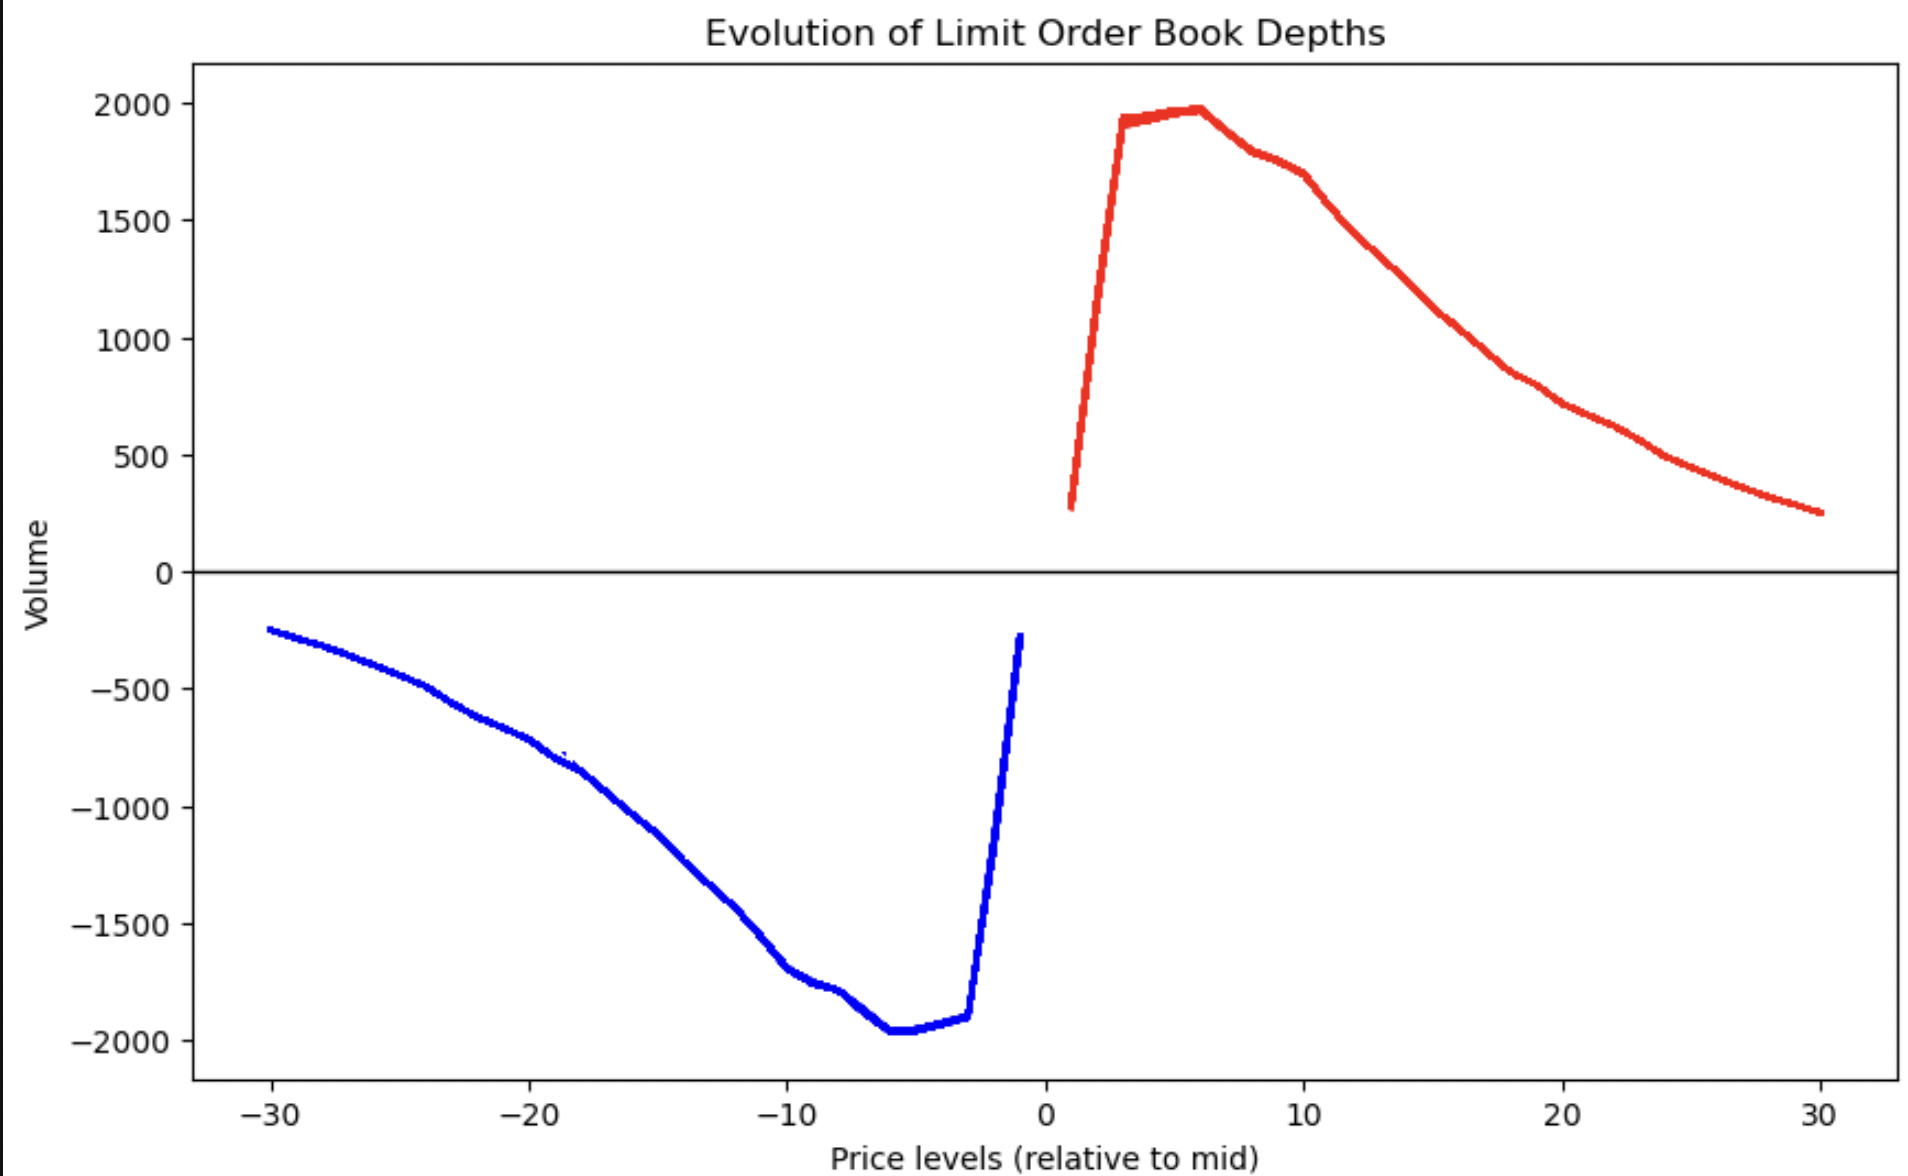
\includegraphics[width=0.82\textwidth]{Screenshot 2025-11-09 at 2.49.05 PM.png}
    \caption{Simulated Average Depth of the Order Book for SCHN.PA w.r.t. the mentioned parameters}
    \label{fig:book-lambda}
\end{figure}
% \begin{figure}[H]
%     \centering
%     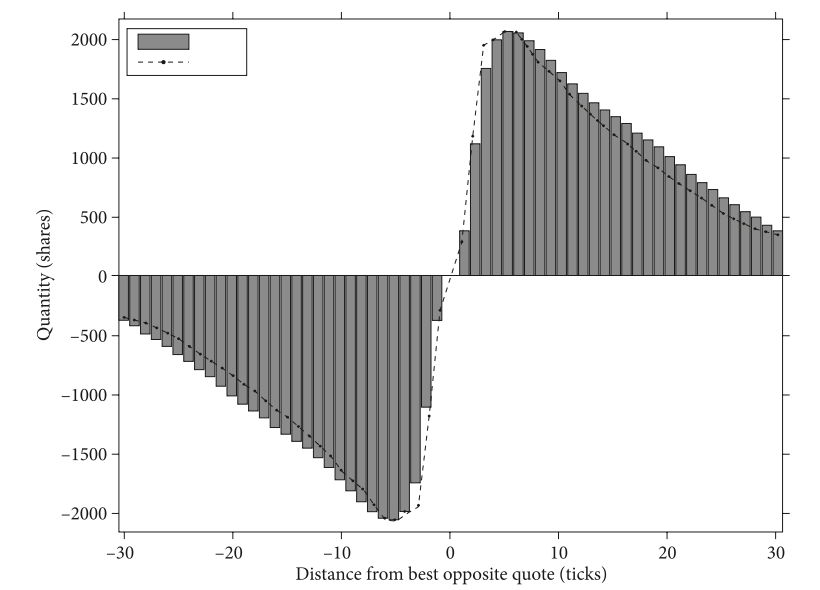
\includegraphics[width=0.82\textwidth]{Screenshot 2025-11-09 at 2.22.28 PM.png}
%     \caption{Average depth profile $\langle X_i \rangle$ as a function of tick distance. as mentioned in \cite{Abergel2016}}
%     \label{fig:book-depth}
% \end{figure}

\section*{Further Simulations}

The reconstruction of the depth profiles in the previous section demonstrates that the
implemented simulator successfully reproduces the qualitative behaviour described in the
reference zero-intelligence models. To further assess the robustness of the calibrated
simulation framework, we extend our analysis to an entirely different dataset by studying
the L10 millisecond-level limit order book of Microsoft (MSFT) on 21 June 2012, obtained
from the LOBSTER database.

\section{Data Description}

The LOBSTER dataset provides message files and limit order book snapshots at user-specified
depth. For a given trading day, the dataset includes:
\begin{itemize}
    \item \textbf{Message File} (matrix of size $N \times 6$): containing the event time,
    event type (submission, cancellation, execution, etc.), order identifier, volume,
    price (in units of \$0.0001), and direction (buy/sell).
    \item \textbf{Order Book File} (matrix of size $N \times (4K)$): containing the
    evolution of the top $K$ bid and ask levels, with associated prices and volumes.
\end{itemize}

Events are timestamped to millisecond precision (and up to nanoseconds for certain
periods), and order book rows correspond exactly to the events listed in the message file,
thus ensuring perfect synchronisation. Unoccupied book levels beyond the available depth
are filled with dummy values following the LOBSTER standard
(\texttt{-9999999999} for bids and \texttt{9999999999} for asks).

Using this structure, we first estimate the model parameters from MSFT data using the
same methodology applied earlier for SCHN.PA, namely:
\[
\lambda^{M} = \frac{N^{M}_{T}}{2T}, \qquad
\lambda^{L}_{i} = \frac{N^{L}_{i,T}}{2T}, \qquad
\lambda^{C}_{i} = \frac{N^{C}_{i,T}}{2T \langle X_{i} \rangle}.
\]

\section{Estimated Parameters}

Applying the above estimators to the MSFT L10 dataset, we obtain the following Poissonian
intensity parameters (buy and sell sides being treated symmetrically due to the large sample
size):
\[
\lambda^{M}_{\text{buy}} = 0.7139776, \qquad
\lambda^{M}_{\text{sell}} = 0.7139776,
\]
\[
\lambda^{L}_{i} = 
\begin{pmatrix}
0.0,\, 2.8007,\, 2.2445,\, 0.6058,\, 0.3152,\, 0.2862,\, 0.2029,\,
0.1307,\, \\0.1258,\, 0.1872,\, 0.1216,\, 0.0213,\, 1.71\times10^{-4},\,\\
6.41\times10^{-5},\, 0.0,\, 6.41\times10^{-5},\, 0,\, \ldots, 0
\end{pmatrix},
\]
and cancellation intensities:
\[
\lambda^{C}_{i} =
\begin{pmatrix}
0.0,\, 2.33\times10^{-4},\, 1.24\times10^{-4},\, 2.96\times10^{-5},\,
1.78\times10^{-5},\, \\ 1.23\times10^{-5},\, 1.18\times10^{-5},\, 
9.26\times10^{-6},\, 1.23\times10^{-5},\, \\ 1.60\times10^{-5},\, 
1.51\times10^{-5},\, 3.86\times10^{-6},\, 4.52\times10^{-5},\, 0,\dots
\end{pmatrix},
\]
with larger cancellation spikes observed at deeper levels, reflecting the empirical behaviour
of MSFT's order flow late in the trading day. Hidden liquidity parameters are set to
\[
a_{\infty} = 250, \qquad b_{\infty} = 250,
\]
consistent with the original zero-intelligence specifications.

\section{Simulated versus Empirical Depth Profiles}

Using the estimated intensity parameters together with the simulation algorithm described
in Section~9.2, we generate synthetic order book depth profiles and compare them with the
empirical MSFT depth computed directly from the LOBSTER dataset.

Despite originating from fundamentally different sources, one being an empirical
millisecond-resolution order book and the other a stylised Poissonian zero-intelligence
model, the two profiles show remarkable qualitative similarity. In both cases:
\begin{itemize}
    \item Liquidity builds steeply near the best quotes,
    \item Depth peaks within a few ticks from the mid-price,
    \item A gradual decline is observed deeper into the book,
    \item Bid and ask curves remain approximately symmetric.
\end{itemize}

These results highlight the surprising effectiveness of the zero-intelligence framework in
capturing the large-scale structural geometry of real-world order books, even when applied
to a highly liquid NASDAQ stock with complex intraday microstructure dynamics.

Figures~\ref{fig:msft-empirical-depth} and \ref{fig:msft-simulated-depth} present the
empirical and simulated depth profiles respectively.

\begin{figure}[H]
    \centering
    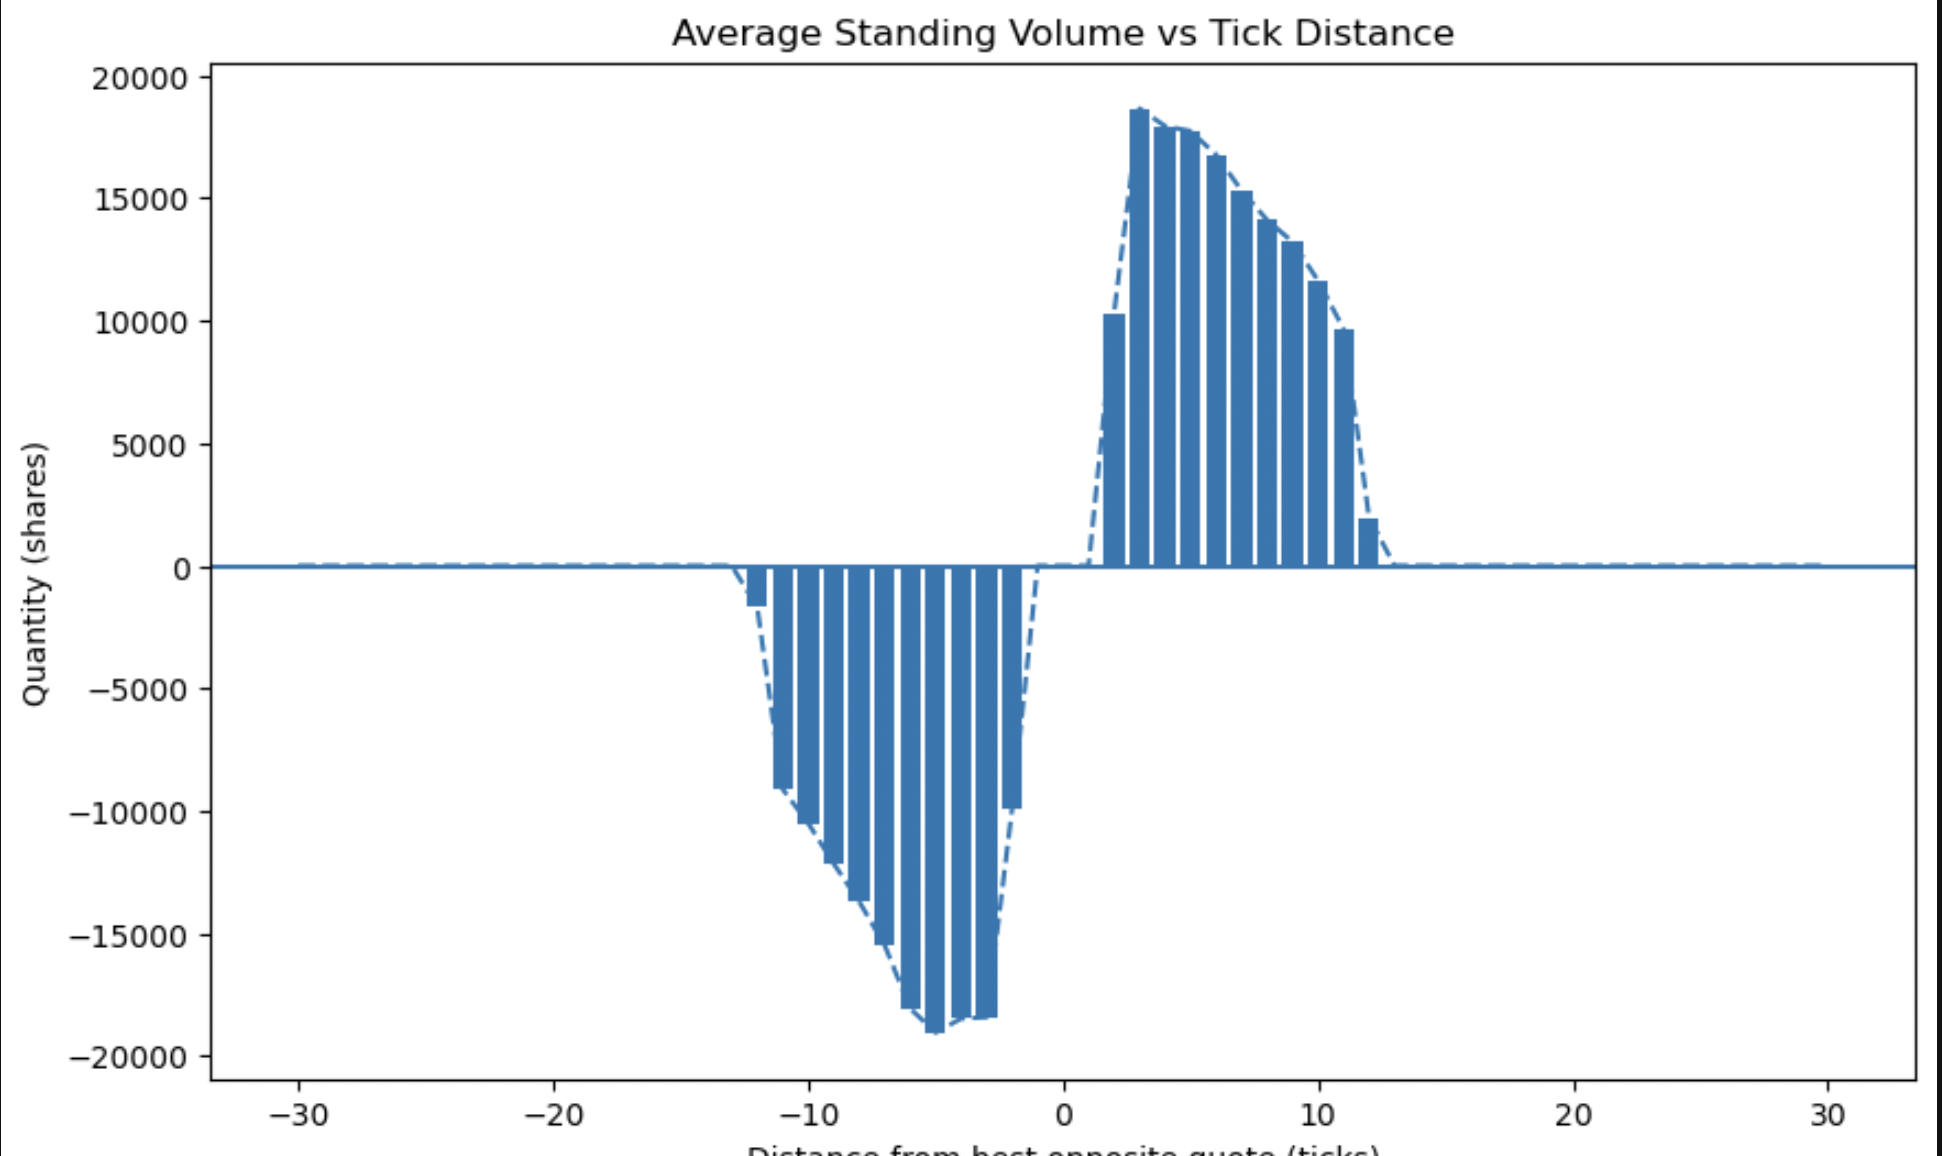
\includegraphics[width=0.82\textwidth]{Screenshot 2025-11-09 at 3.12.06 PM.png}
    \caption{Empirical depth profile of MSFT (21 June 2012) computed from LOBSTER L10 data.}
    \label{fig:msft-empirical-depth}
\end{figure}

\begin{figure}[H]
    \centering
    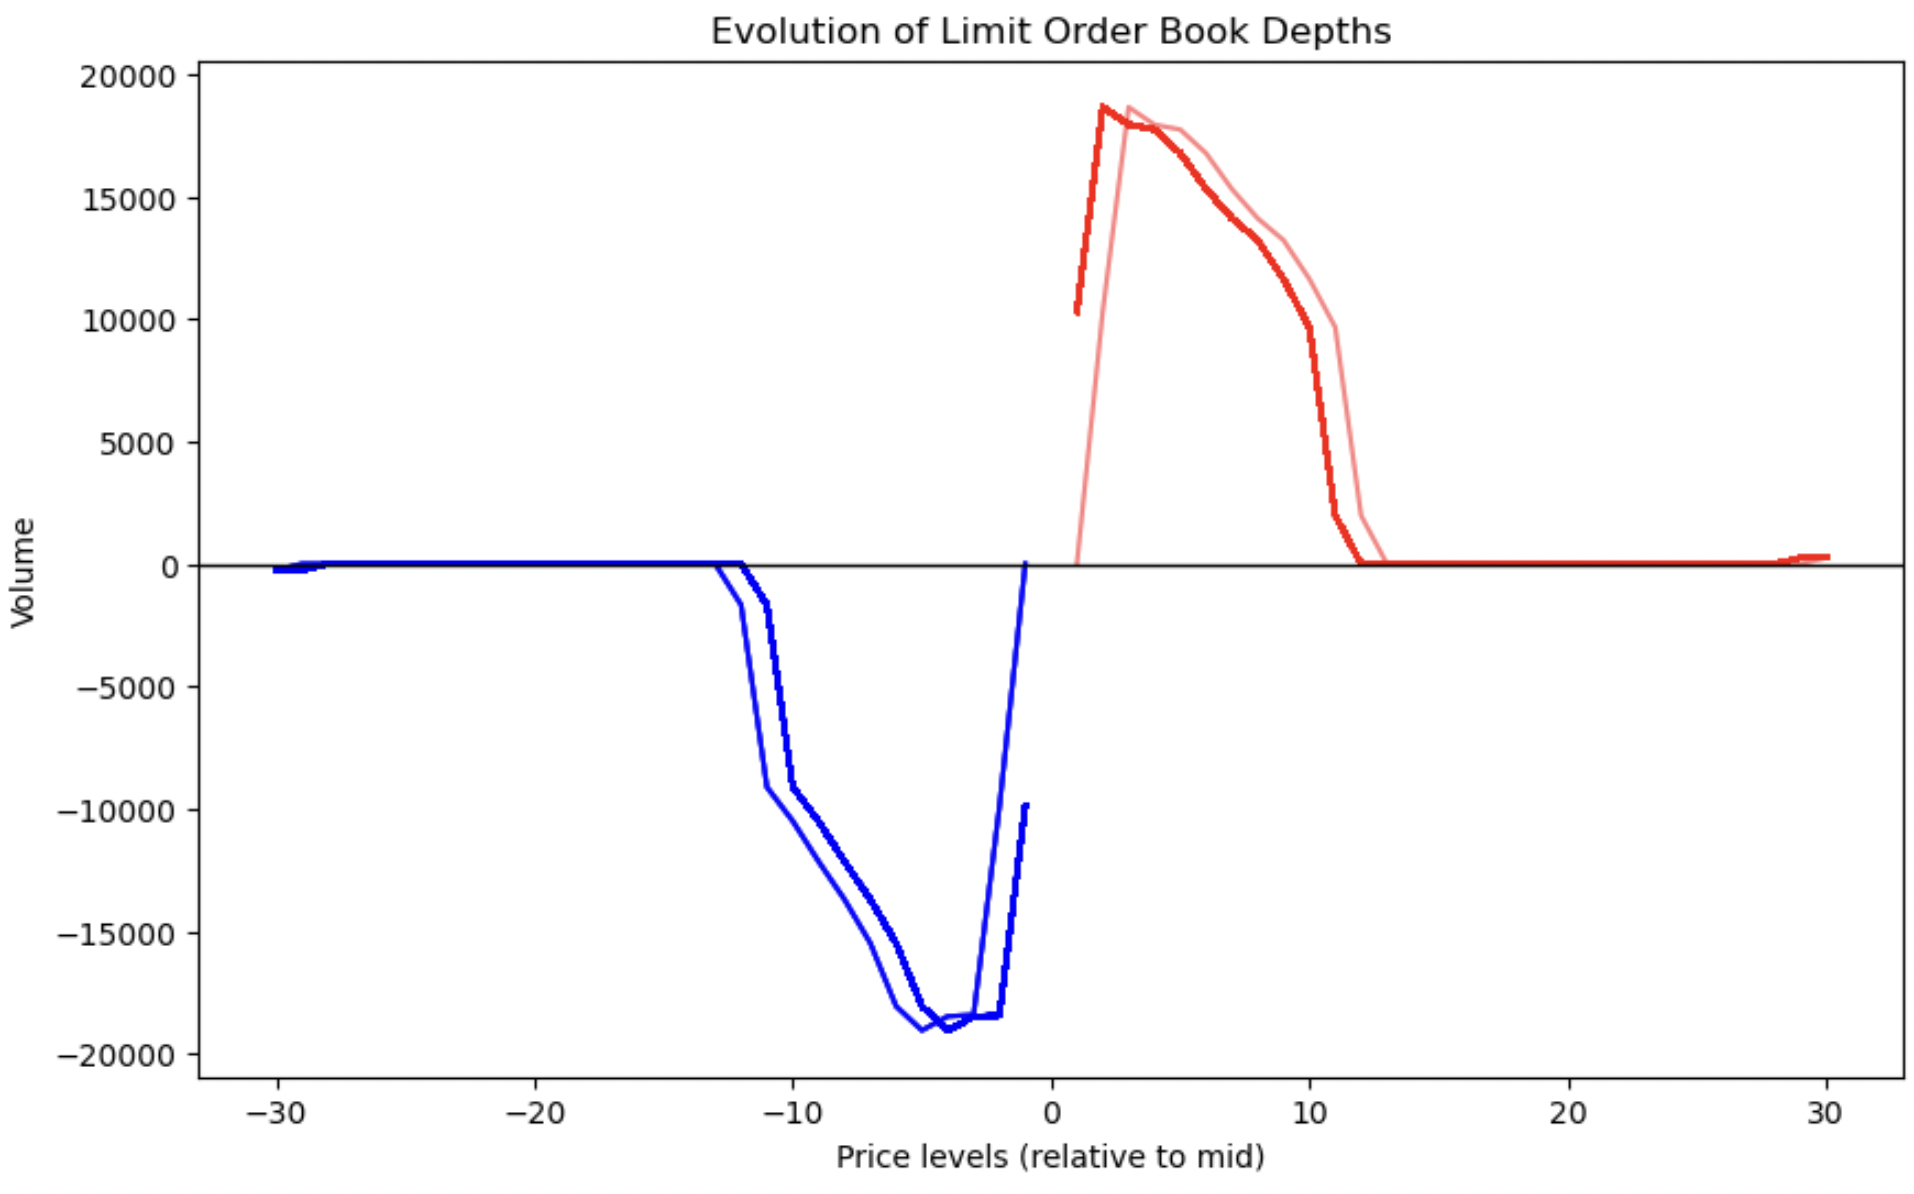
\includegraphics[width=0.82\textwidth]{Screenshot 2025-11-09 at 3.12.28 PM.png}
    \caption{Simulated depth profile for MSFT using parameters estimated from the LOBSTER data.}
    \label{fig:msft-simulated-depth}
\end{figure}

The close alignment between the empirical and simulated structures strengthens the
conclusion that the model, despite its simplicity, encodes sufficient microstructural features
to replicate realistic order book behaviour across different assets and market conditions.
